\begin{figure}[ht]
	\centering
	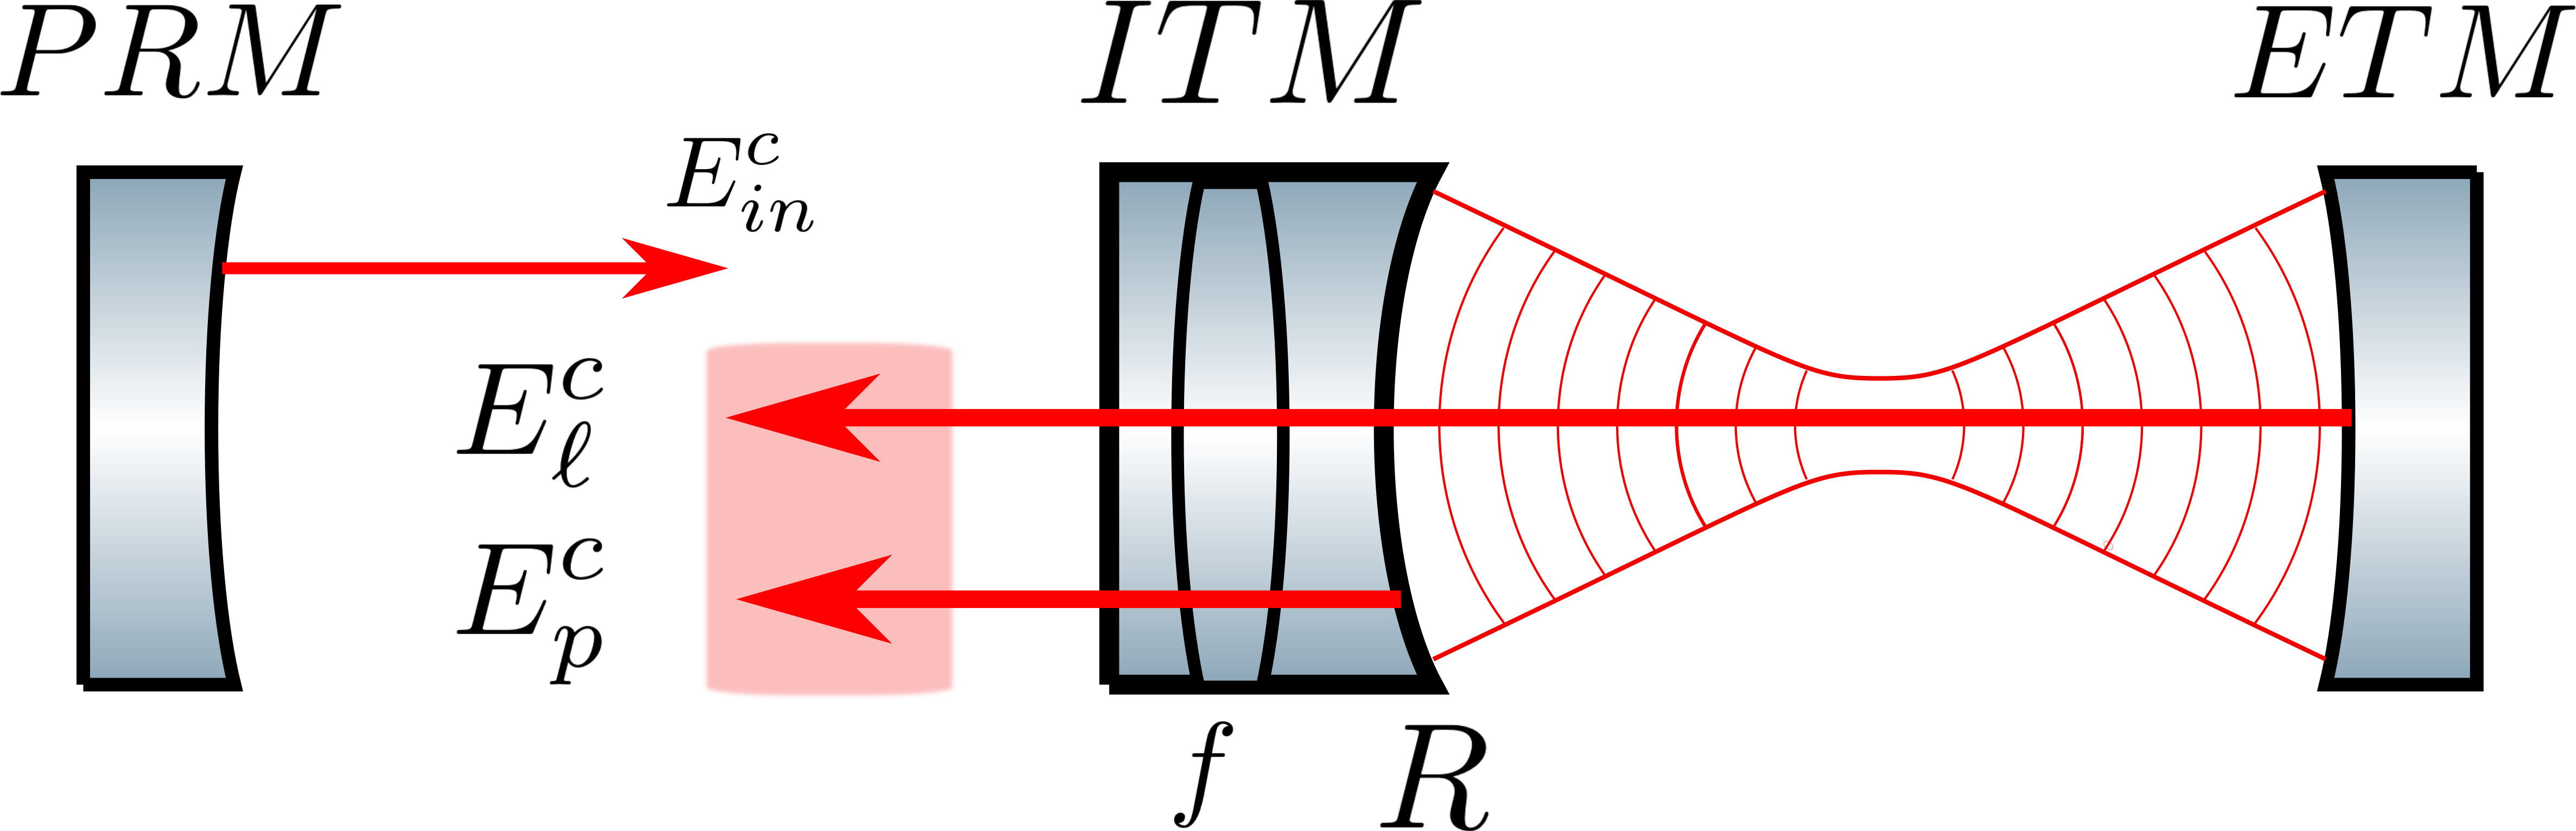
\includegraphics[width=.7 \textwidth]{../Figures/ThermalLensFP.png}
	\caption[A simplified model for the effect of a substrate thermal lens on the carrier field.]  
	{\textbf{A simplified model for the effect of a substrate thermal lens on the carrier field.} An input beam, $E_{\text{in}}^{c}$, from the power recycling mirror (PRM) will have a radius of curvature that mode matches to the input test mass (ITM).  The promptly reflected beam, $E_{p}^{c}$, is denoted by equation \ref{eq:promptE} and the leakage beam, $E_{\ell}^{c}$, is expressed by equation \ref{eq:leakE} where the sum of them would make the total reflected beam.}
	\label{fig:ThermalLensFP}
\end{figure}

\begin{figure}[ht]
	\centering
	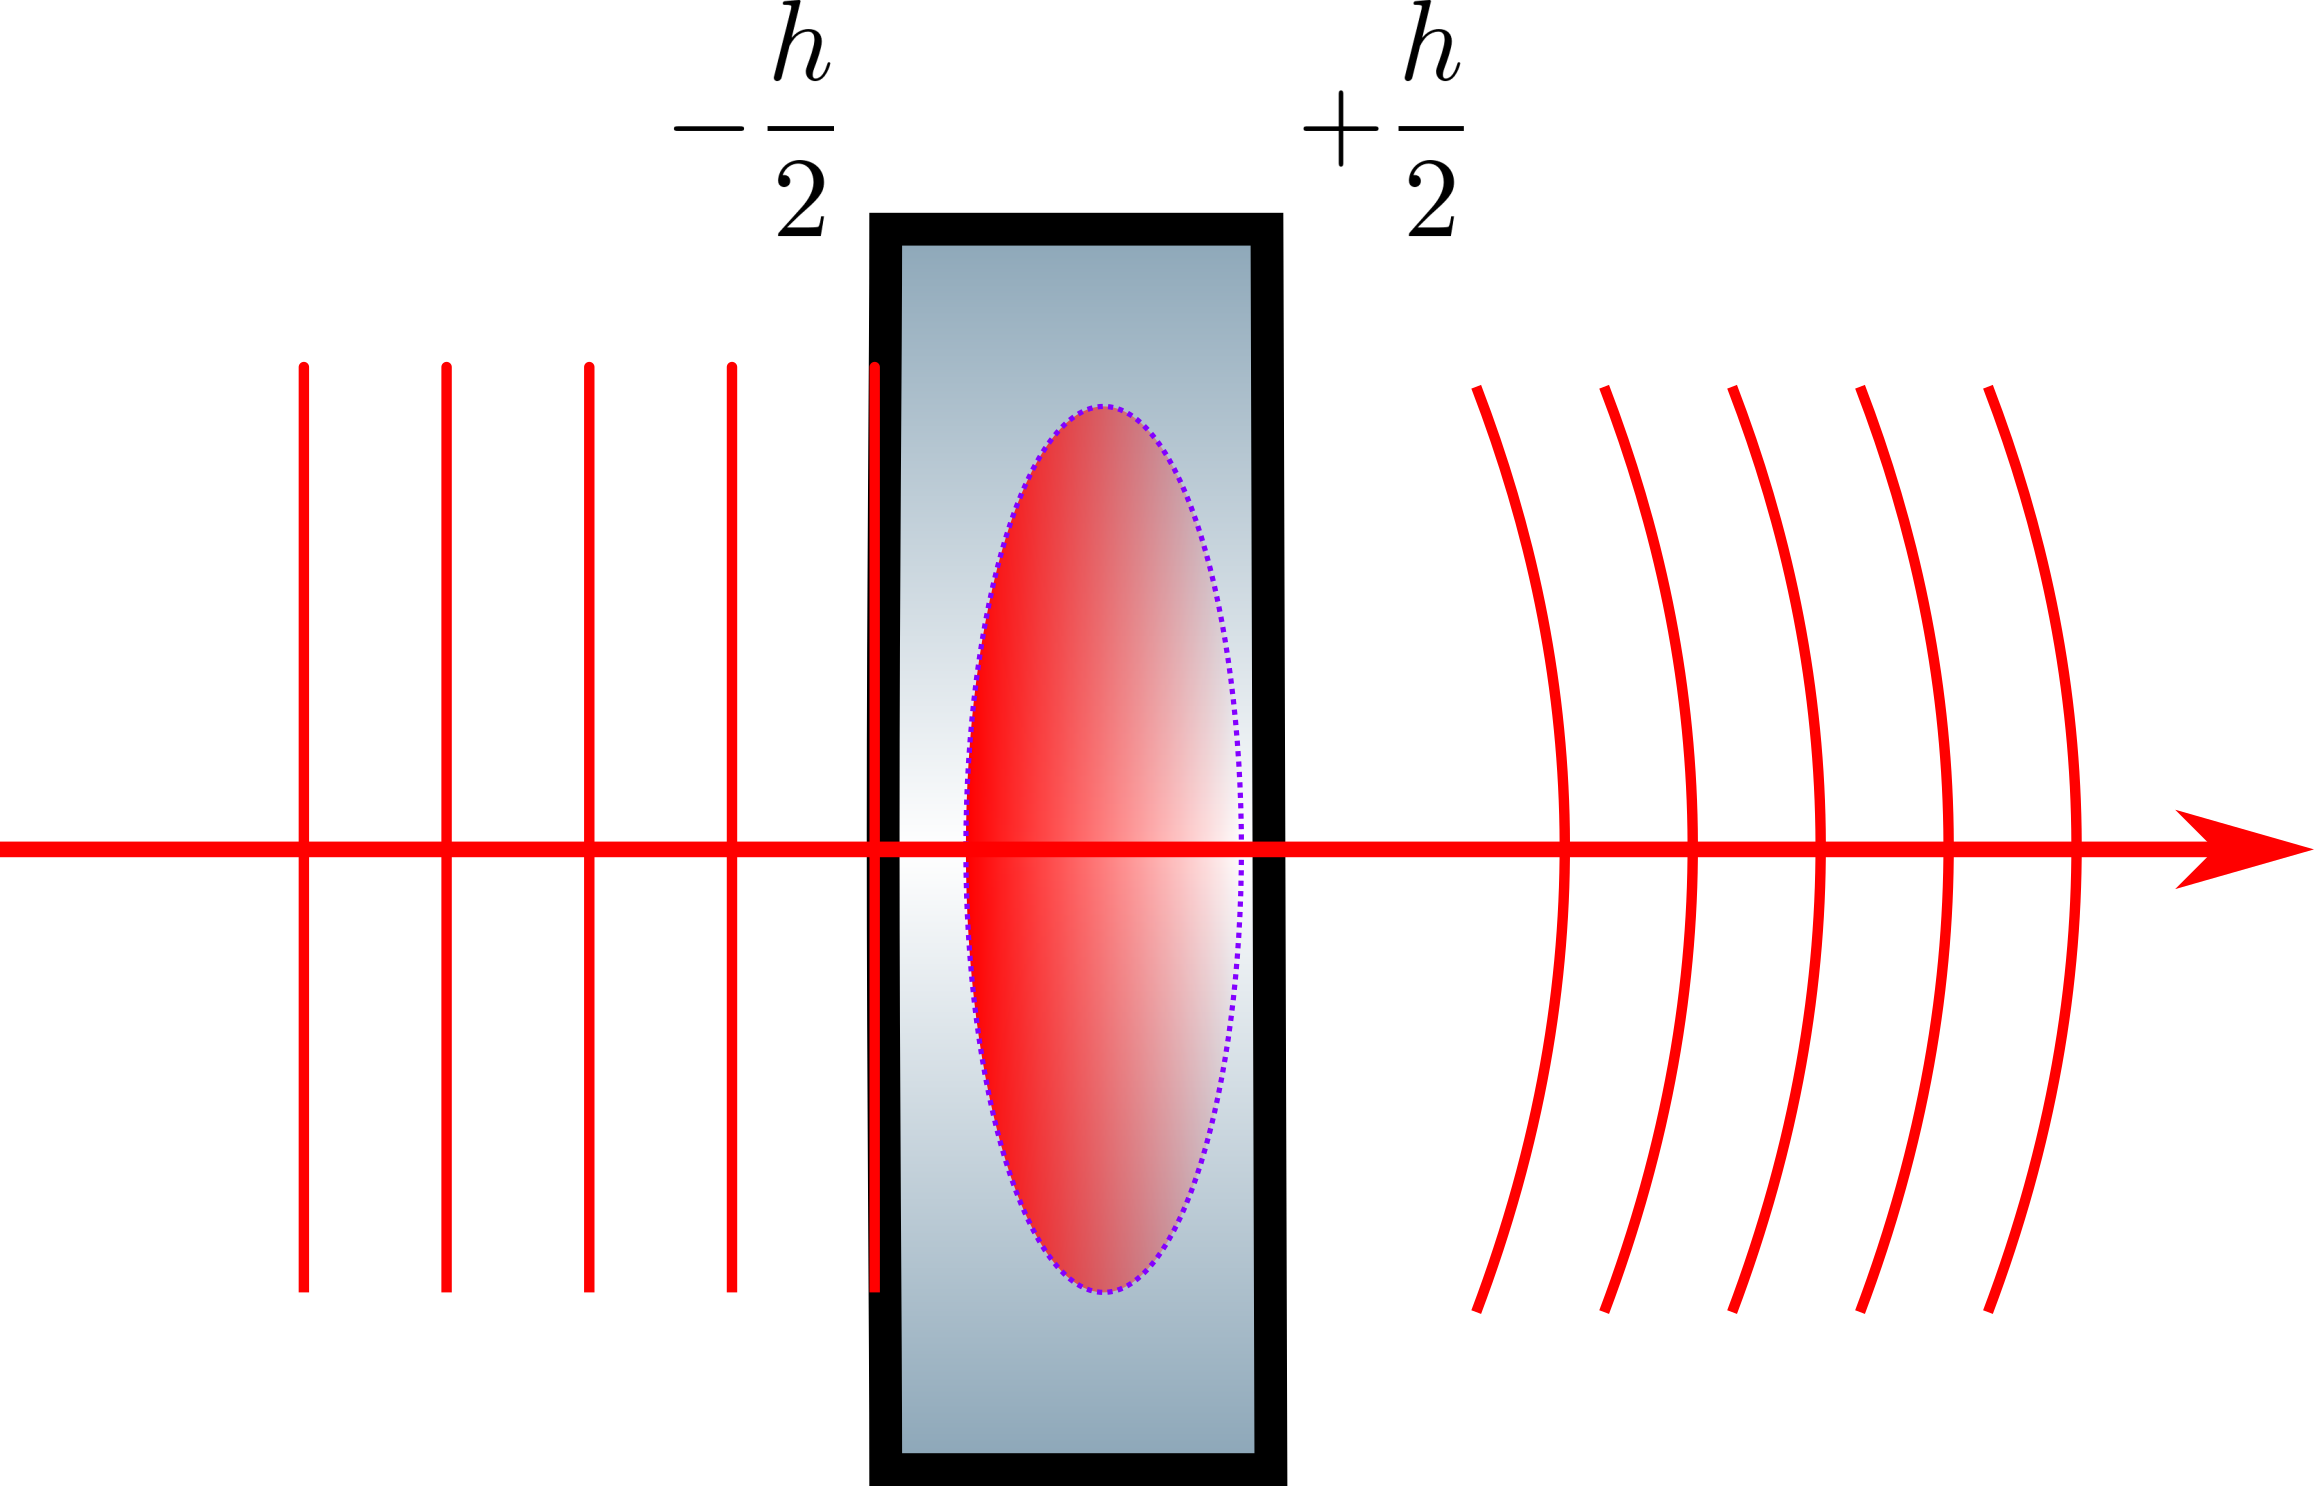
\includegraphics[width=.4 \textwidth]{../Figures/ThermalLensWF.png}
	\caption[A plane wave passing through a lens with a temperature gradient.]  
	{\textbf{A plane wave passing through a lens with a temperature gradient.} The index of refraction, $n$, depends on the material and temperature field, when a plane wave moves through such a lens, then a phase lag or lead occurs in the wavefront. Since $\frac{\text{d}n}{\text{d}T}$ is negative, the thermal distortion will resemble a diverging lens.}
	\label{fig:ThermalLensWF}
\end{figure}

\begin{figure}[ht]
	\centering
	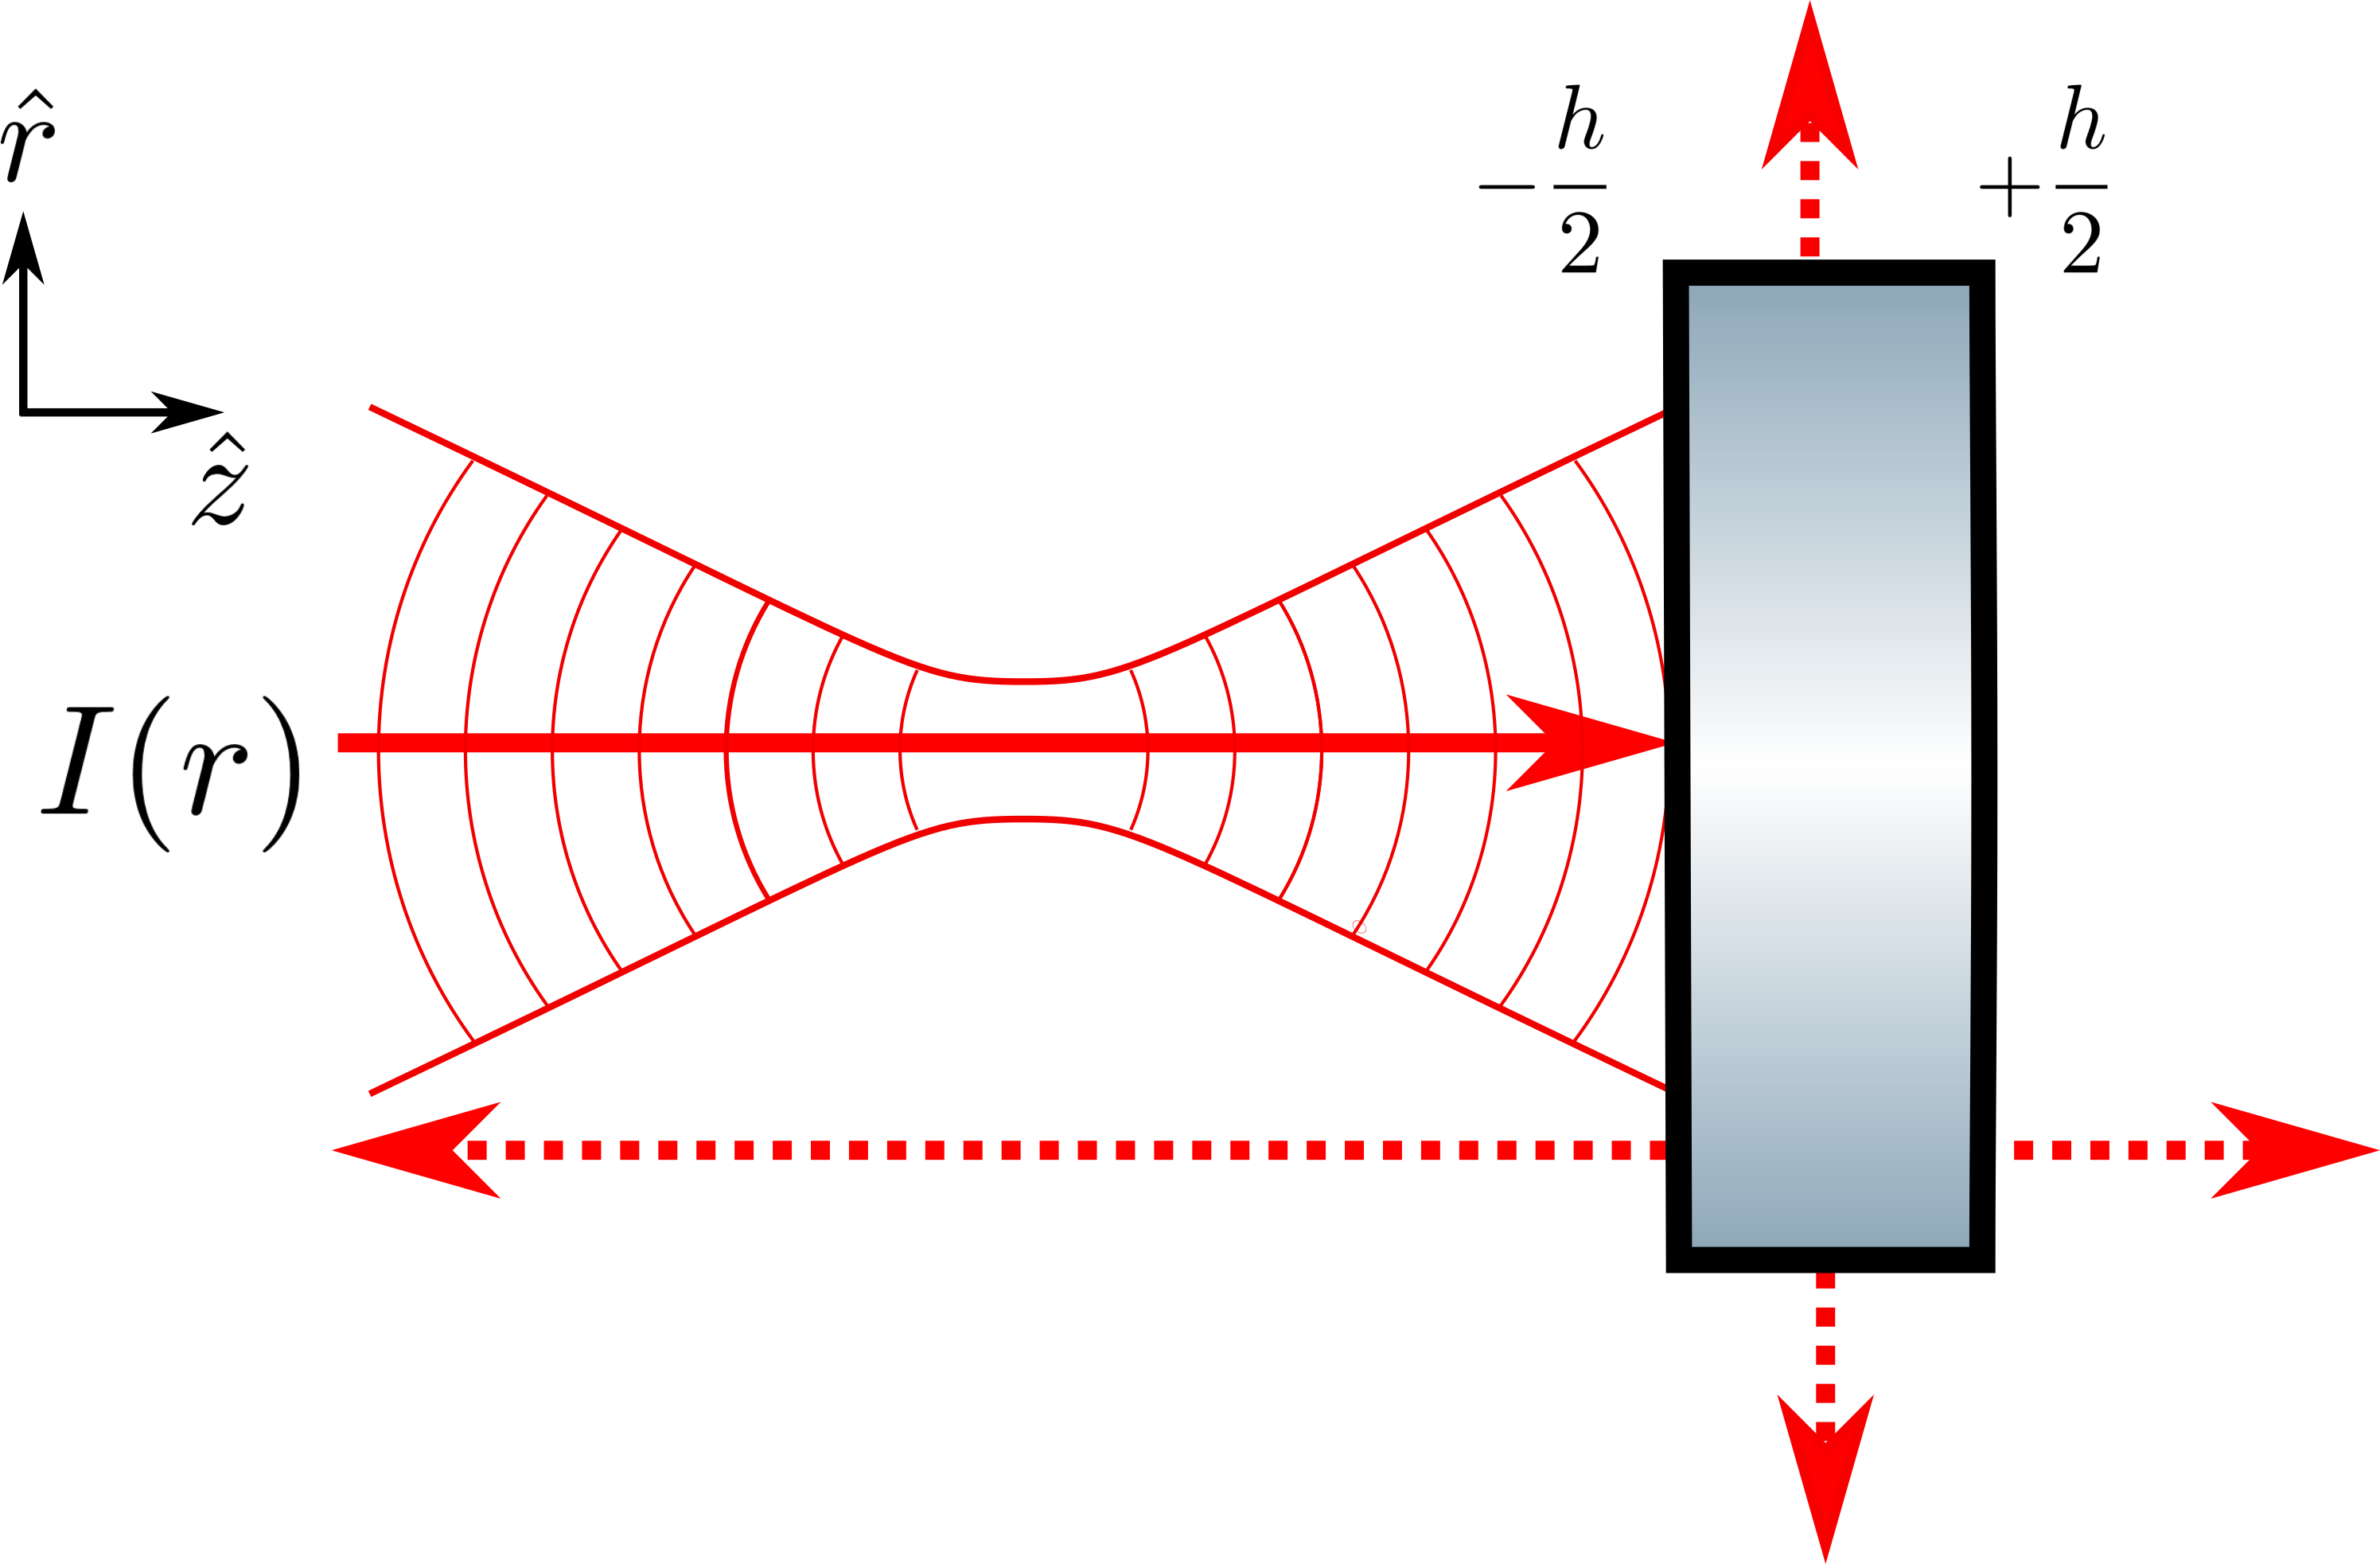
\includegraphics[width=.6 \textwidth]{../Figures/ThermalLensFlux.png}
	\caption[A conceptual model of flux balance for a cylindrical object.]  
	{\textbf{A conceptual model of flux balance for a cylindrical object.} The red dotted lines represent the radiative fluxes escaping the optic while a Gaussian beam with intensity profile $I(r)$ is pumping energy in as denoted by the red solid line.}
	\label{fig:ThermalLensFlux}
\end{figure}

\begin{figure}[ht]
\centering
\begin{subfigure}[a]{0.7\textwidth}
	\centering
	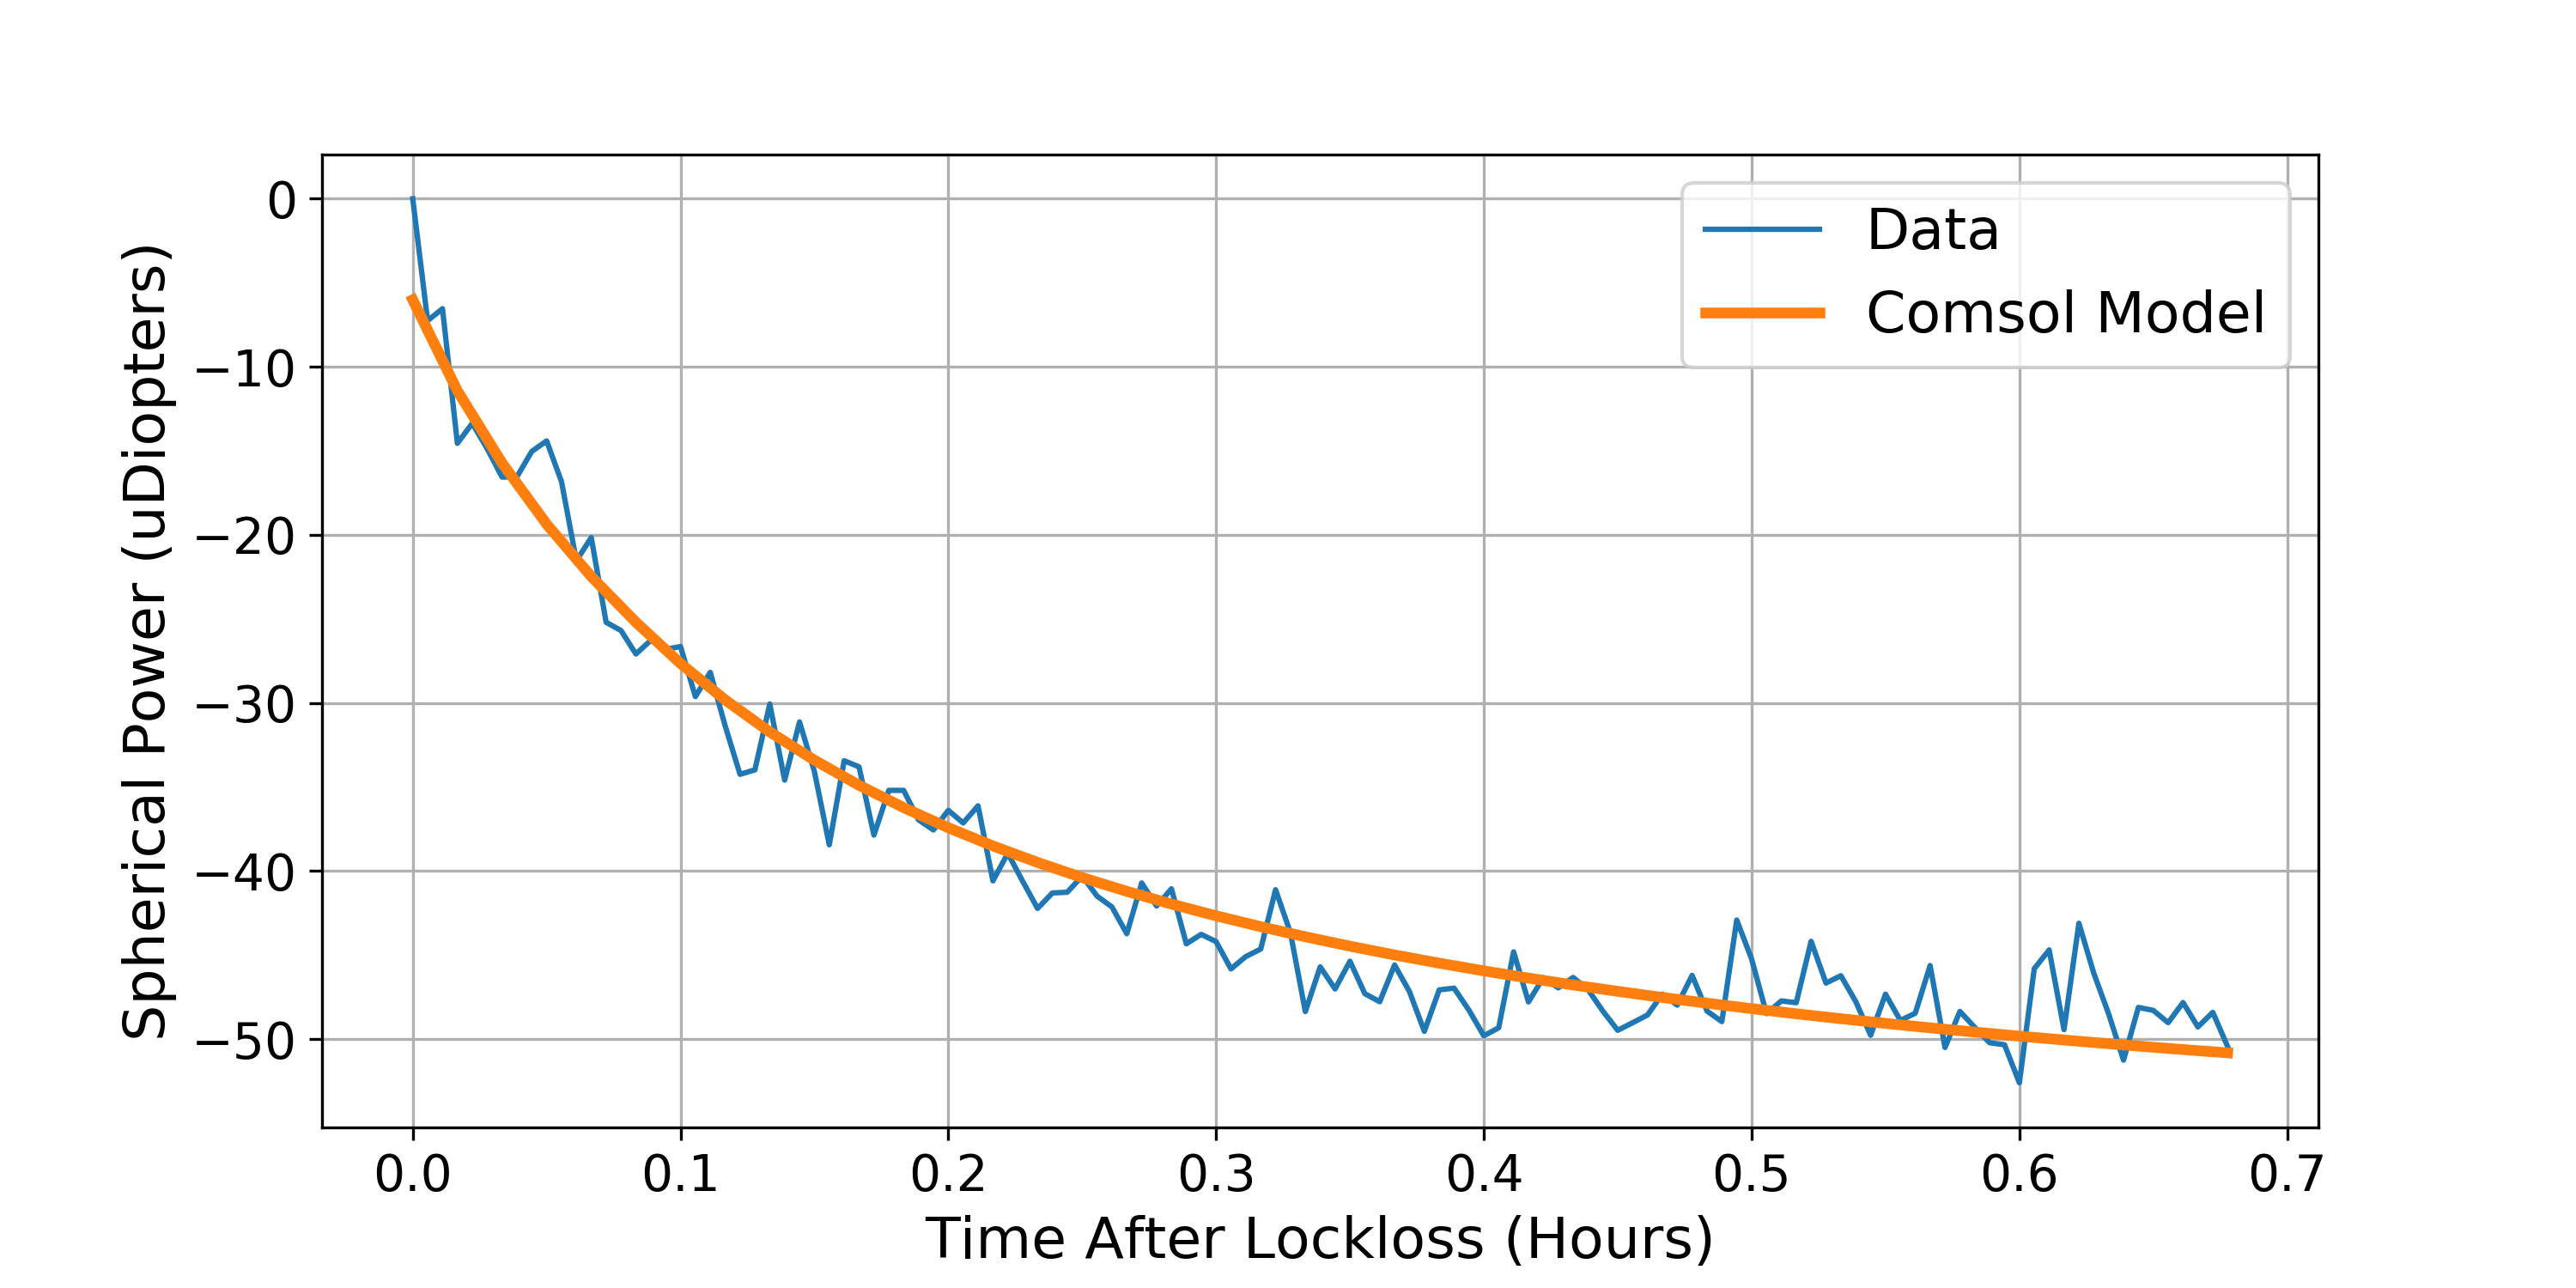
\includegraphics[width=\textwidth]{../Figures/itmx_HWS_Absorption.png}
	\caption{ITMX absorption}
	\label{fig:itmx_abs}
\end{subfigure}
\hfill
\begin{subfigure}[b]{0.7\textwidth}
	\centering
	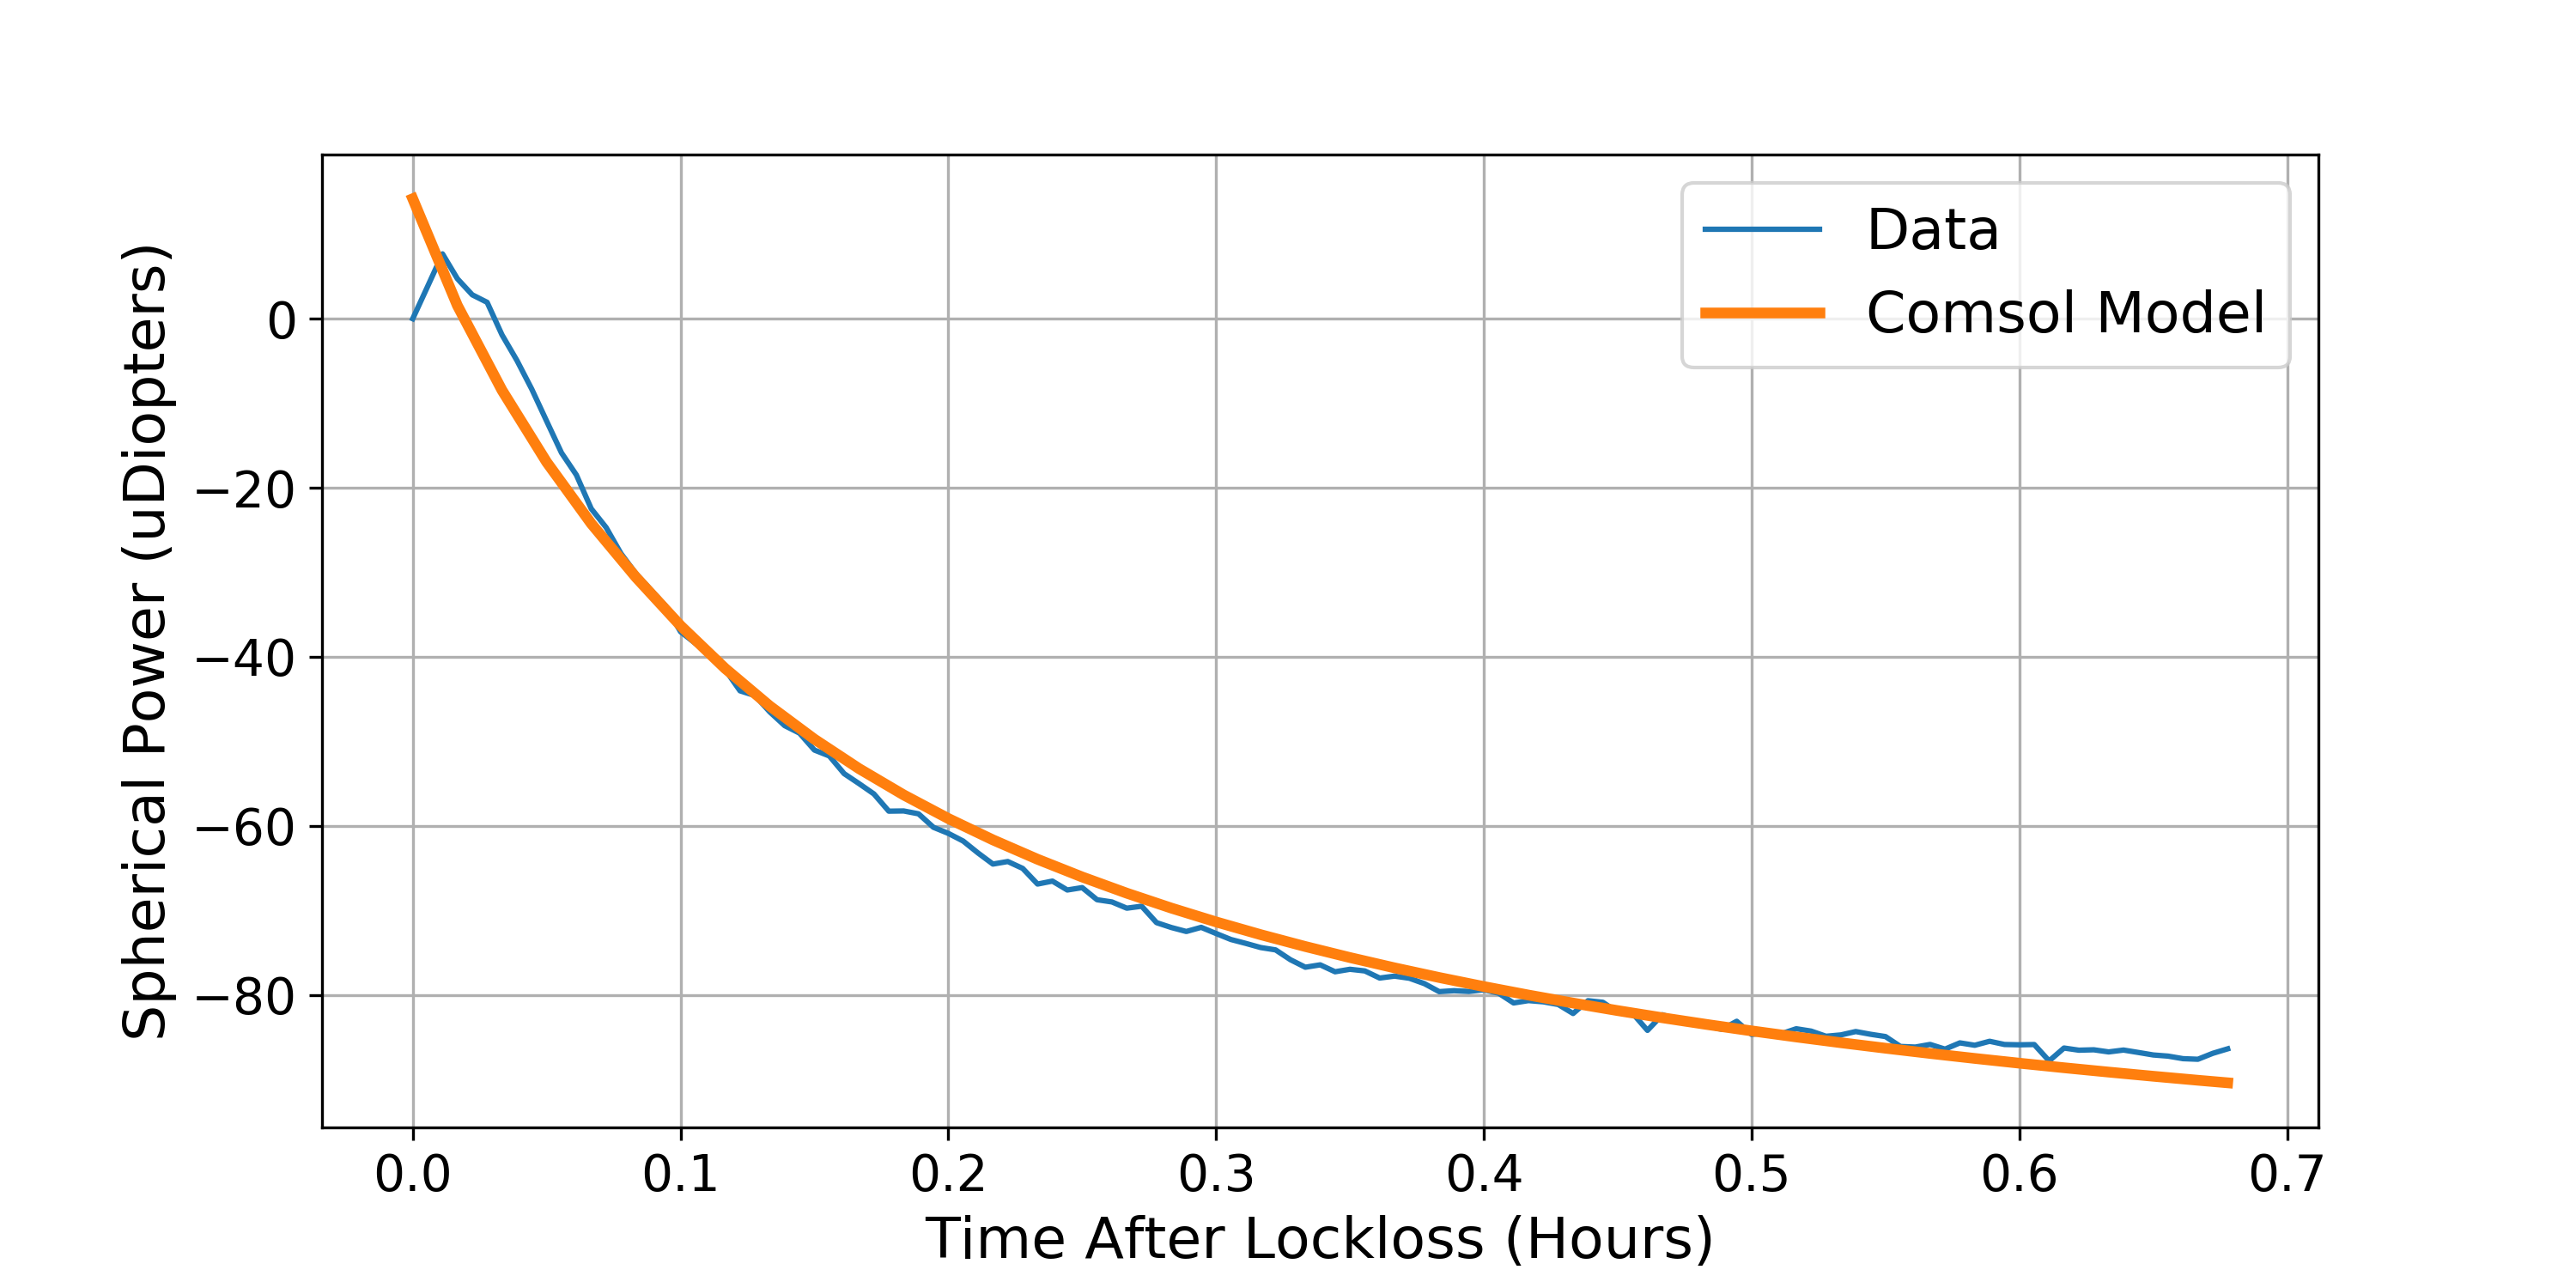
\includegraphics[width=\textwidth]{../Figures/itmy_HWS_Absorption.png}
	\caption{ITMY absorption}
	\label{fig:itmy_abs}
\end{subfigure}
\caption{The amount of spherical lensing from a Gaussian beam is shown by Hello and Vinet \cite{Vinet_Thermal_Issues} and this provides a model which to fit the data.}
\label{fig:hws_abs}
\end{figure}

\begin{figure}[ht]
	\centering
	\begin{subfigure}[b]{1.0\textwidth}
		\centering
		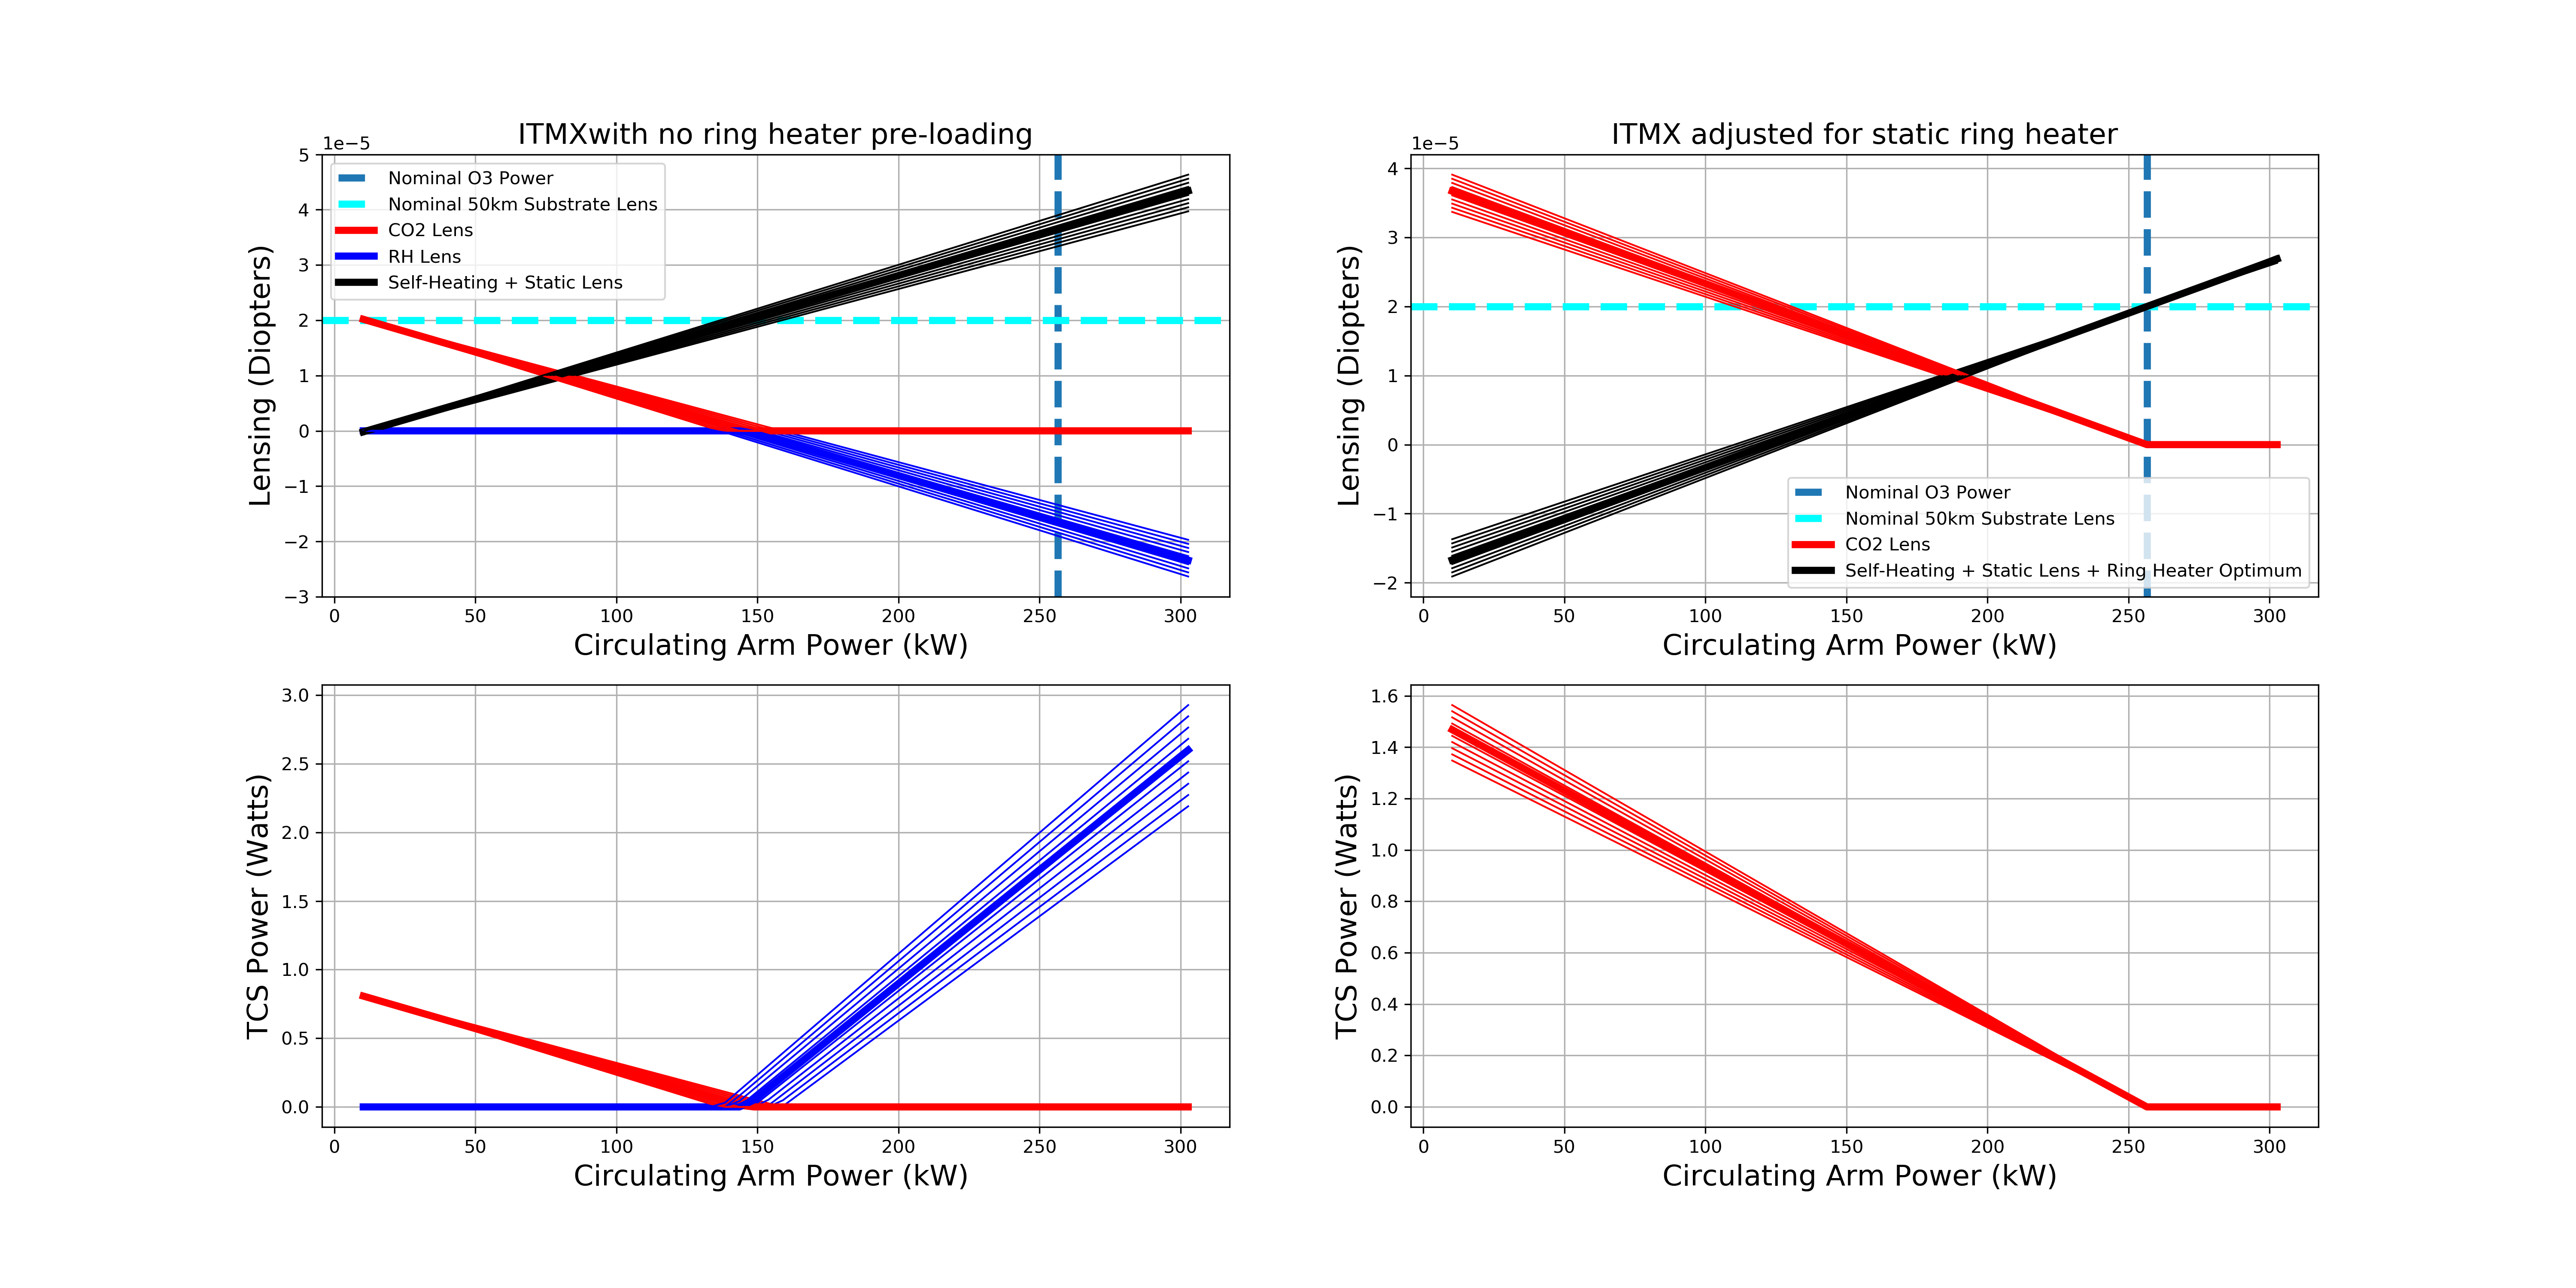
\includegraphics[width=\textwidth]{../Figures/ITMX_TCS_Settings.png}
		\label{fig:TCS_ITMX}
	\end{subfigure}
	\hfill
	\begin{subfigure}[b]{1.0\textwidth}
		\centering
		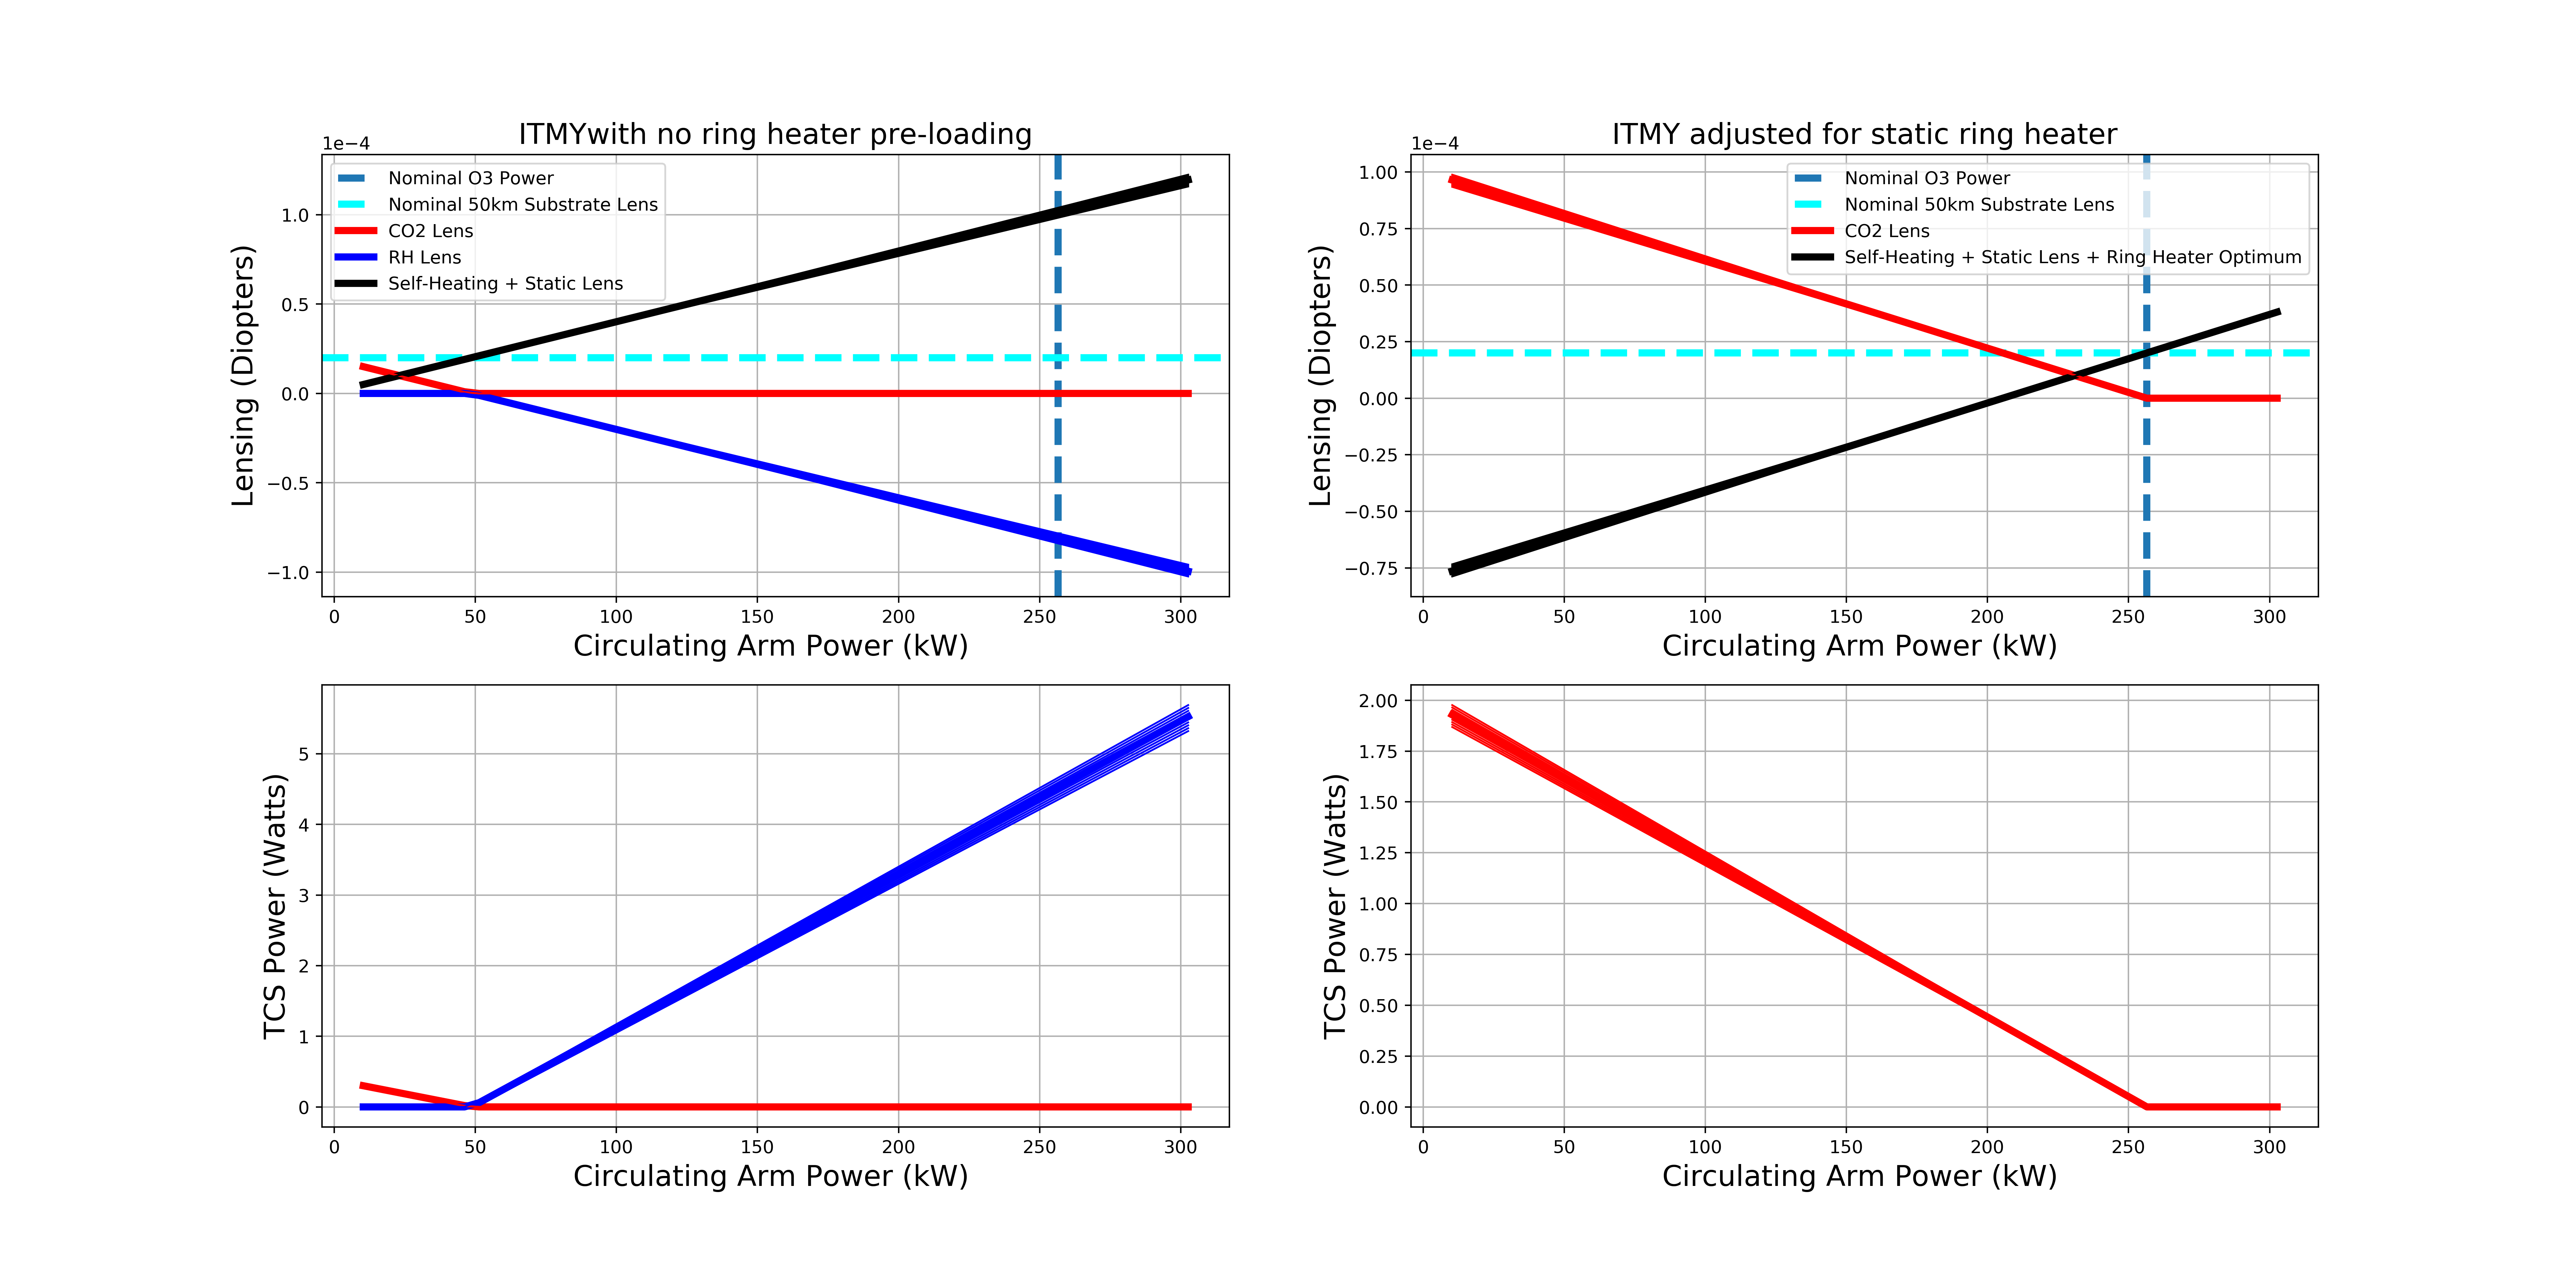
\includegraphics[width=\textwidth]{../Figures/ITMY_TCS_Settings.png}
		\label{fig:TCS_ITMY}
	\end{subfigure}
	\caption[Calculated TCS settings to balance the substrate lens.]{
		\textbf{Calculated TCS settings to balance the substrate lens.}  The nominal circulating power denoted by the vertical blue line is a function of the input power, the recycling gain, and the arm cavity gain.  The nominal input power for O3 will be 50 Watts and the power recycling gain is around 45.  The arm cavity gain can be estimated by calibrating the transmitted power from each of the arms and is approximately 228.  The horizontal, dashed turquoise line represents the nominal substrate lens with a focal length of 50 km.  This value is what the power recyling cavity expects to properly mode match to the arms. }
	\label{fig:TCS_ITMs}
\end{figure}

\begin{figure}[ht]
\centering
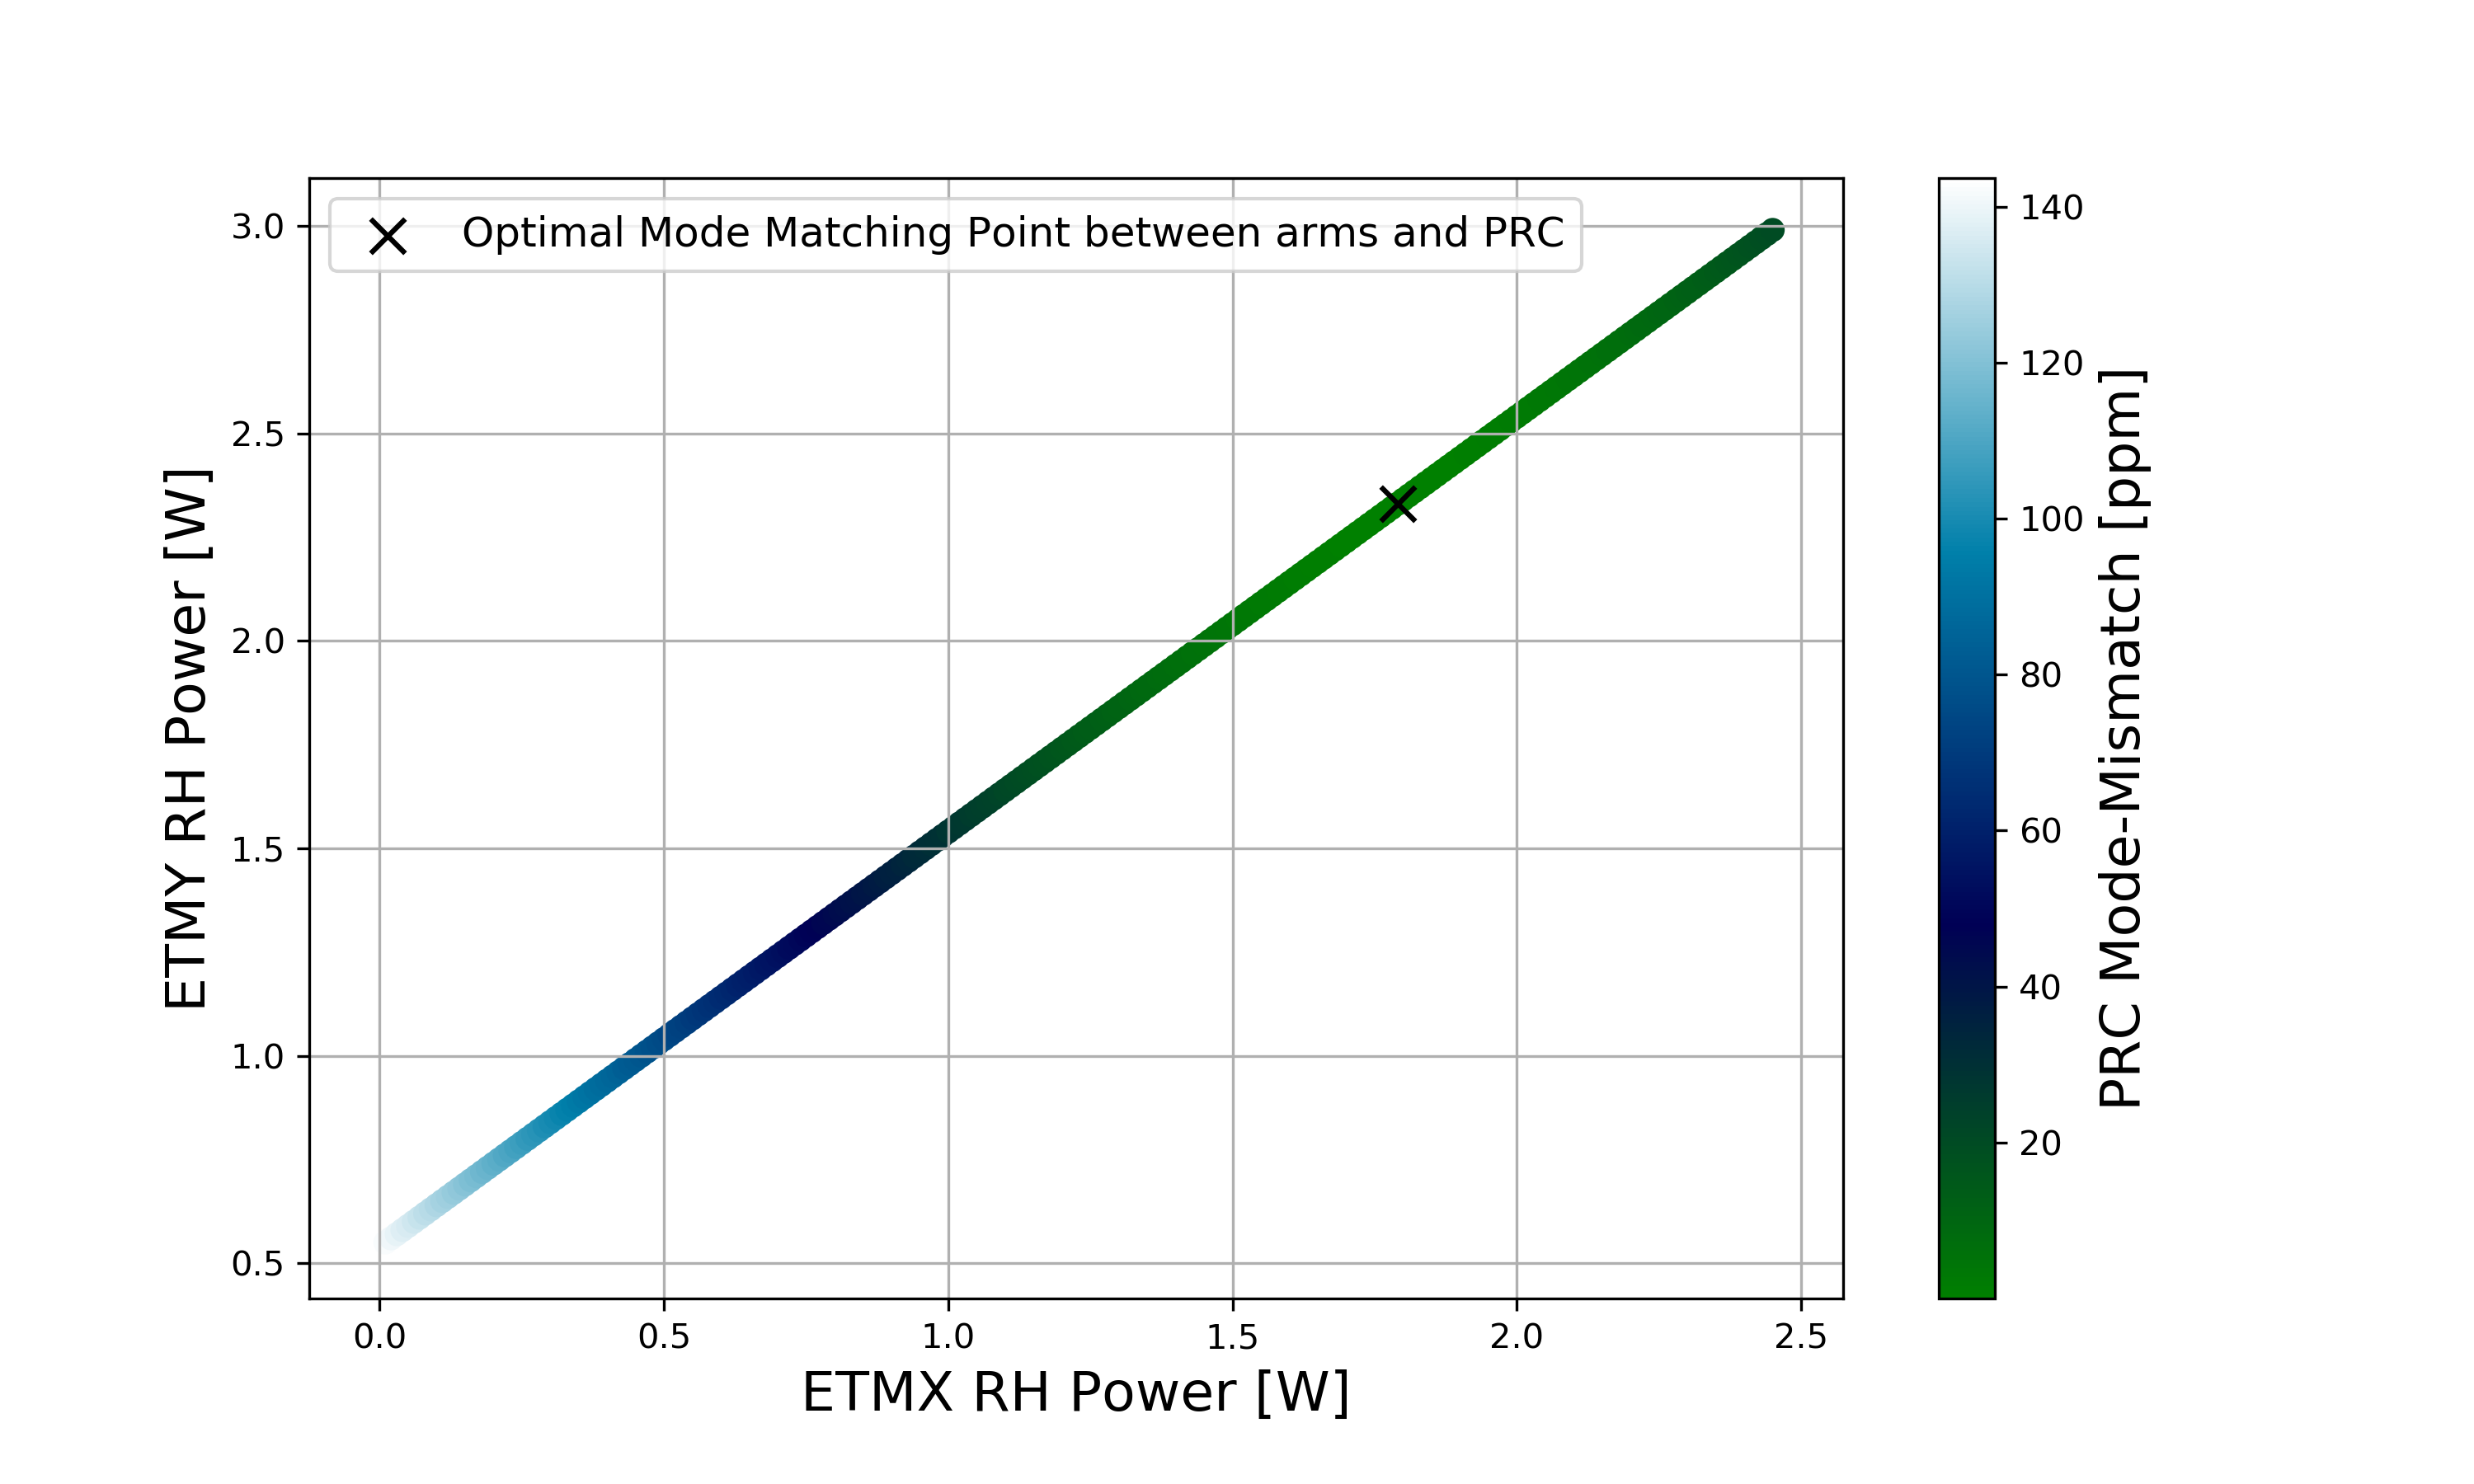
\includegraphics[width=1.0 \textwidth]{../Figures/ETM_TCS_Settings.png}
\caption[Mode matching the arm cavities to the power recycling cavity.]{
	\textbf{Mode matching the arm cavities to the power recycling cavity.}  Determining the ring heater and CO2 settings still leaves the end test mass ring heaters to be set.  The goal is to maintain the mode matching between the arms while simultaneously searching for the optimal overlap with the power recycling cavity. The linear portion of the graph shows a combination of common and differential adjustment of each ring heater that keeps the mode matching between the arms at less than 1 ppb, }
\label{fig:TCS_ETM}
\end{figure}

\begin{figure}[ht]
	\centering
	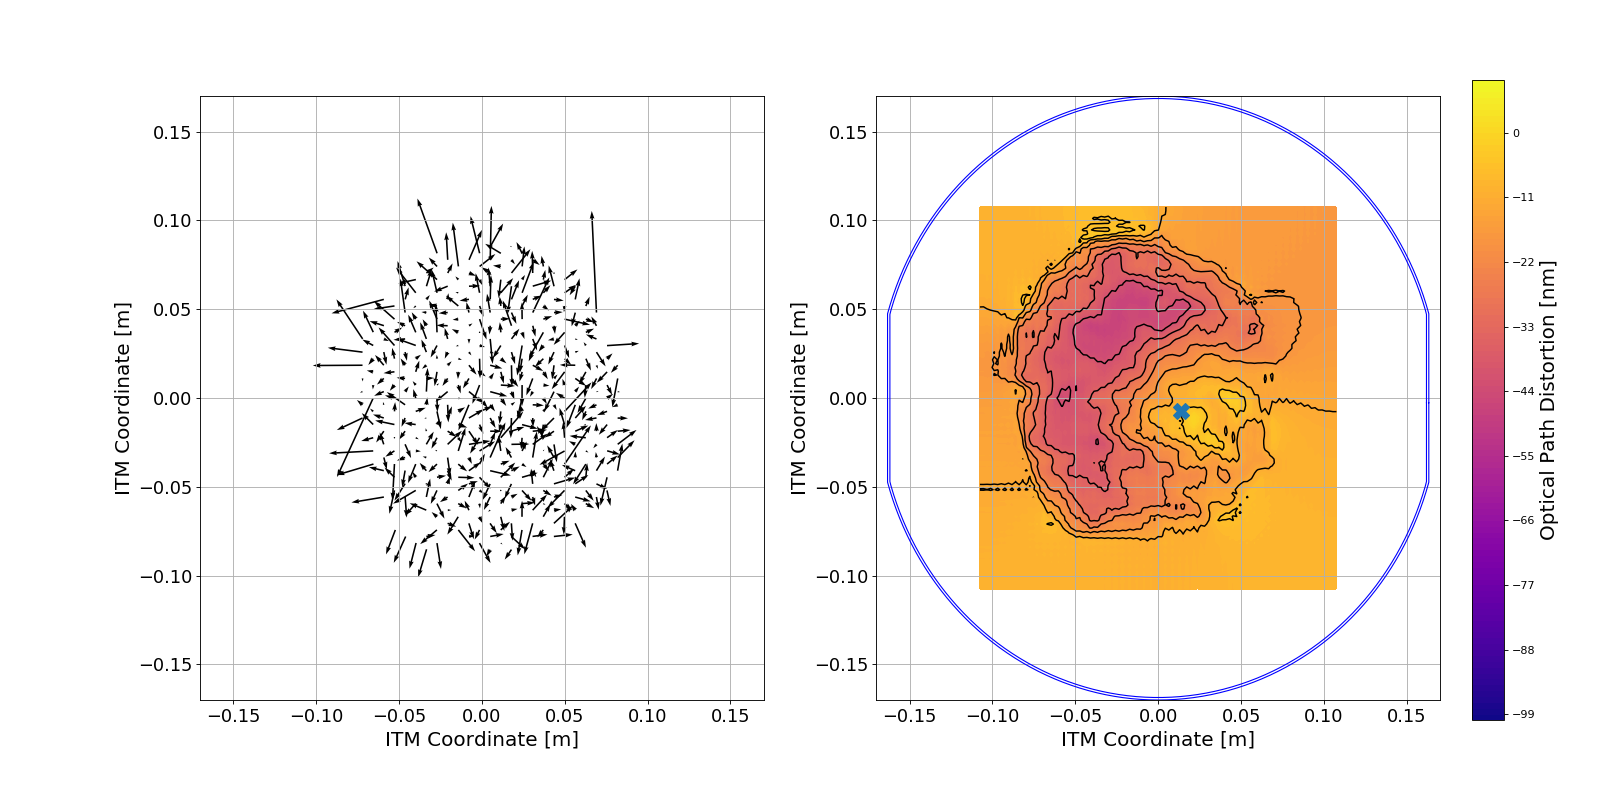
\includegraphics[width=.7 \textwidth]{../Figures/ITMX_20W_abs.png}
	\caption[A wavefront map measured by the Hartmann Wavefront Sensor of ITMX.]  
	{\textbf{A wavefront map measured by the Hartmann Wavefront Sensor of ITMX.}}
	\label{fig:ITMX_WF}
\end{figure}

\begin{figure}[ht]
	\centering
	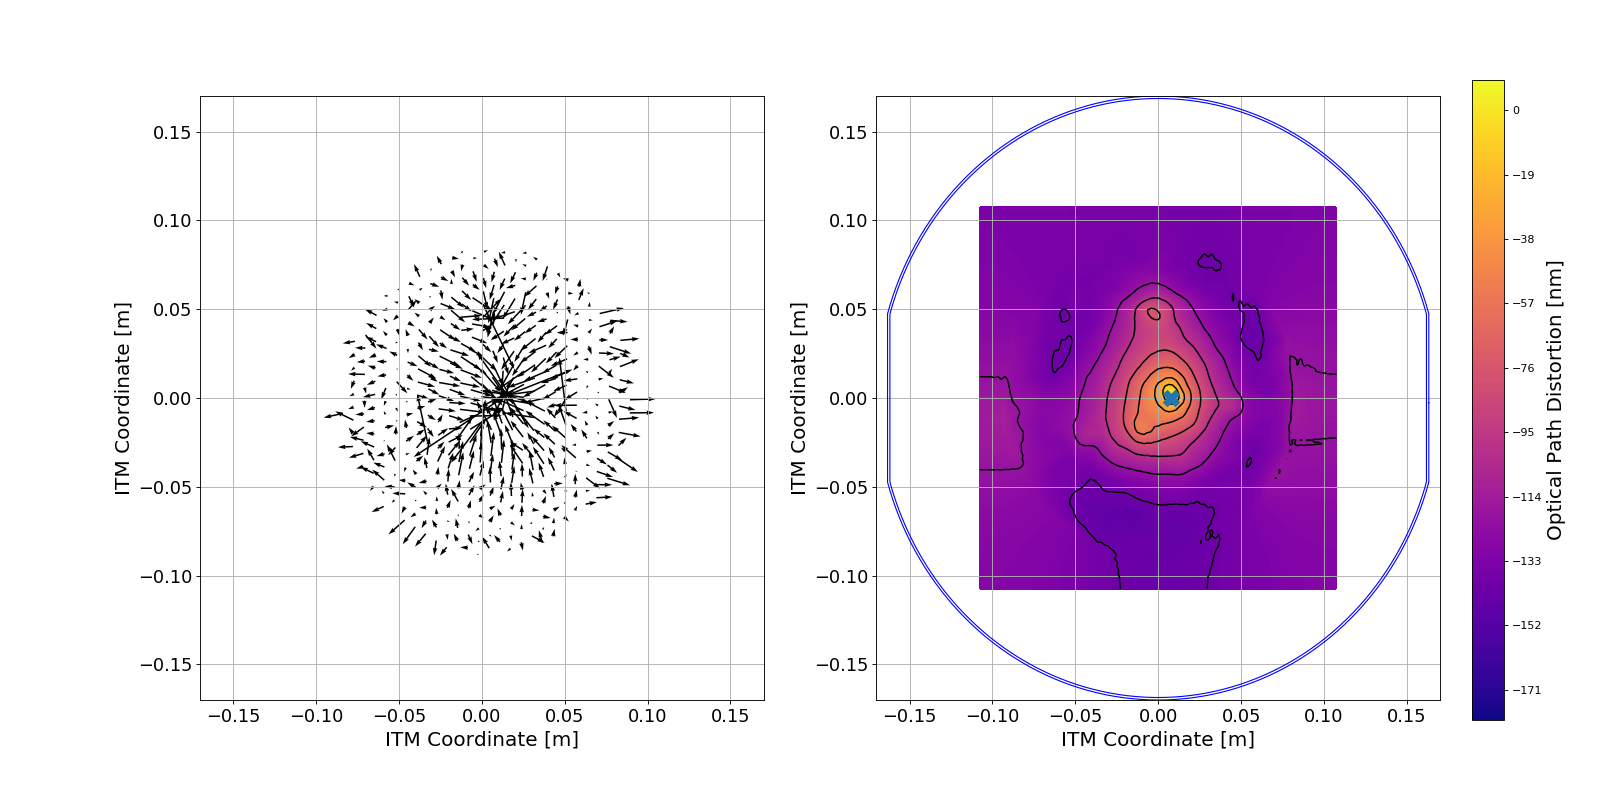
\includegraphics[width=.7 \textwidth]{../Figures/ITMY_20W_abs.png}
	\caption[A wavefront map measured by the Hartmann Wavefront Sensor of ITMY.]  
	{\textbf{A wavefront map measured by the Hartmann Wavefront Sensor of ITMY.}}
	\label{fig:ITMY_WF}
\end{figure}
